\section{Experiment 1: Can AI Generate Exam Questions? Five Blind Rounds, \textyen13.87}
\label{sec:exp1}

\subsection{Question}
The product needs an ``internalization'' route: instead of reusing the bank, can a generative model write new chemistry items that a student cannot distinguish from examination items? We treated this as a measurement problem, not a capability question, and ran five rounds.

\subsection{Protocol}
Anchor items from the R5 pool; human blind judgments of distinguishability under adversarial pairwise comparison; a cost audit per round; explicit dead/alive verdict per route.

The judge is the author. This is a single-judge protocol, not an expert panel; we state it plainly because it bounds the strength of the finding (Section~\ref{sec:limitations}). The judgment set spans 153 items across three rounds: 60 from-scratch, 53 style-transfer, 40 second-round style-transfer; plus $>$70 figure-anchored items verified by direct inspection. Items were presented in randomized within-pair order; the judge was blind to route and generation round, and only the counting rule (did the judge classify the generated item as real?) was post-hoc. No inter-rater agreement statistic is available by construction; the per-route binomial one-sided 95\% lower bounds are: from-scratch $\geq$77\%, style-transfer $\geq$51\% (60\% fair-condition subset: $\geq$43\%). We report the raw label tables rather than only summary percentages so the reader can recompute.

\begin{table}[h]
\centering
\small
\begin{tabular}{lll}
\toprule
\textbf{Route} & \textbf{Measurement} & \textbf{Verdict} \\
\midrule
From-scratch & 87\% distinguishable & \textbf{dead} (practice only) \\
Style transfer & 65\% / 60\% fair & \textbf{alive} (high-fidelity) \\
Programmatic rendering & passes & live, scalable \\
Figure-anchored reskin & $\approx$26/29 pass & \textbf{alive} \\
\bottomrule
\end{tabular}
\caption{Five-round generation verdicts.}
\label{tab:exp1}
\end{table}

\subsection{Results and the boundary}
From-scratch generation was dead: 87\% of items were distinguishable, twice (two rounds identical), and the marginal gain from a third attempt was measured at zero. Figure~\ref{fig:generation} summarizes the route-level measurements. Style transfer survived: 65\% distinguishable under adversarial comparison, 60\% under fair conditions---still above chance, but a real working band. The product rule that followed: \emph{generated items never enter the diagnostic path}.

\begin{figure}[t]
\centering
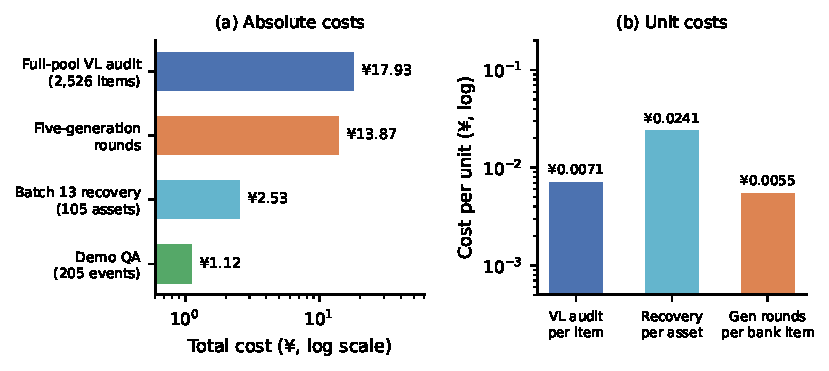
\includegraphics[width=\textwidth]{figures/fig6_costs.pdf}
\caption{Measured costs of the evidence pipeline: absolute (a) and per-unit (b). Note the log scales.}
\label{fig:costs}
\end{figure}

\begin{figure}[t]
\centering
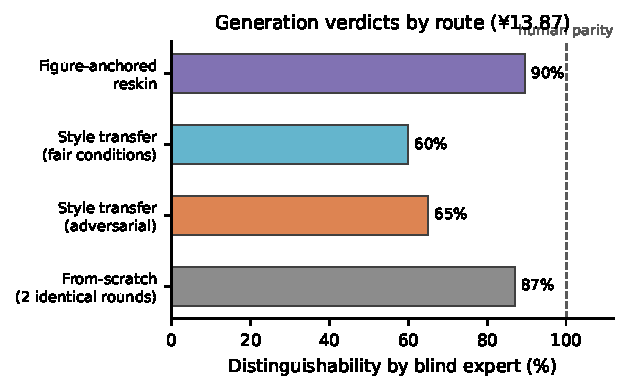
\includegraphics[width=0.6\textwidth]{figures/fig3_generation.pdf}
\caption{Five-round generation verdicts. Distinguishability by blind expert under adversarial pairwise comparison. The dashed line marks human parity.}
\label{fig:generation}
\end{figure}



Figure~\ref{fig:costs} places the audit costs in context. The five rounds cost \textyen13.87 in total; this is API and tooling spend, not compensated human review---the blind judgments were contributed by the author without payment.

\subsection{Why this matters for the genre}
Three meta-lessons, each recorded as a product rule:
\begin{enumerate}\setlength{\itemsep}{0pt}\setlength{\parskip}{0pt}\setlength{\parsep}{0pt}
\item \textbf{Adversarial distinguishability is not student-scenario serviceability.} A generated item can be both more distinguishable and more usable than a real item; these are different orders.
\item \textbf{Generators inherit the corpus's transcription scars.} When the reference bank itself has residual defects (ion subscripts, figures), generation reproduces them and adds new ones.
\item \textbf{Goodhart is a property of any acceptance rule.} Every acceptance line must anchor to non-forgeable concrete objects---numeric values, IDs, hashes---never to semantic interpretation.
\end{enumerate}

\subsection{Against the literature}
Published blinded evaluations of AI-generated multiple-choice items often find judges perform at or near chance (51.4\% source identification in \cite{nursing2025}; 69.2\% and 73.6\% of participant ratings for the two highlighted exercise questions wrongly rated as Human in \cite{chatgptqg2025}; blinded medical panels rating GPT-4 items comparable to expert human items in overall impression, with higher rates of items unfit for use \cite{medicalteacher2025}); under item-response-theory analysis, prompted generation can produce items with human-like difficulty and discrimination \cite{anaquest2025}. Our 87\%/65\% numbers are higher. We attribute this to (a) examination-specific fidelity of the reference set (real Shanghai items have distinctive surface signatures: multi-step compound reasoning, figure-anchored stems, standardized answer keys) and (b) the private gold-label protocol that governs ours. We do not generalize: this is a measurement on one examination system.
